\documentclass[10pt,a4paper]{article}

%──────────────────────────────────────────────────────────────────────────────
% Packages
%──────────────────────────────────────────────────────────────────────────────
\usepackage[a4paper,margin=1in]{geometry}
\usepackage{helvet}
\renewcommand{\familydefault}{\sfdefault}

\usepackage{graphicx}
\usepackage{booktabs}
\usepackage{array}
\usepackage{caption}
\usepackage{wrapfig}
\usepackage{parskip}
\usepackage{amsmath}
\usepackage[numbers]{natbib}
\usepackage{hyperref}

\captionsetup{font={small,it},labelfont={small,it},skip=4pt}

\setlength{\parindent}{0pt}
\setlength{\parskip}{6pt}

\title{\vspace{-3.2cm}\fontsize{14}{16}\selectfont\textbf{Benchmarking six deep learning reconstruction models for sparse view photoacoustic tomography}}

\author{{%
\fontsize{11}{13}\selectfont
$^{1}$Yash Thakre, $^{2}$Mridul Verma, $^{2}$Partha Pratim Pal, $^{2,*}$Renu John\\[6pt]
\fontsize{9}{12}\selectfont 
$^{1}$Department of Biotechnology, \\ 
National Institute of Technology Warangal, Telangana, India\\[4pt]
$^{2}$Department of Biomedical Engineering, \\ 
Indian Institute of Technology Hyderabad, Telangana, India\\[5pt]
\textit{$^{*}$renujohn@bme.iith.ac.in}%
}}

\date{}

\begin{document}

\maketitle
\vspace{-25pt}
\thispagestyle{empty}

%──────────────────────────────────────────────────────────────────────────────
%──────────────────────────────────────────────────────────────────────────────
{\itshape
Photoacoustic Tomography (PAT) combines optical contrast with ultrasonic resolution for biomedical imaging. Sparse-view acquisition produces severe reconstruction artifacts when conventional methods are used. Limited-view acquisition introduces severe artifacts when conventional Filtered Back-Projection (FBP) is used, motivating deep-learning-based reconstruction methods capable of restoring fine structural details.
}

\vspace{6pt}

We compare six representative reconstruction models using three different strategies. U-Net and FD-UNet operate on reconstructed images, with FD-UNet employing dense skip connections for improved feature propagation. Y-Net, FD-YNet, and AS-Net jointly utilize reconstructed images and raw acoustic measurements, while AS-Net incorporates attention-based feature fusion. DeepMB adopts a model-based projection framework that reconstructs directly from measurement data while preserving the underlying physical information. All models were trained and evaluated on the OADAT dataset using the 128-element sensor configuration, ensuring a consistent experimental setup for fair performance comparison.

%──────────────────────────────────────────────────────────────────────────────
\begin{figure}[h]
\centering
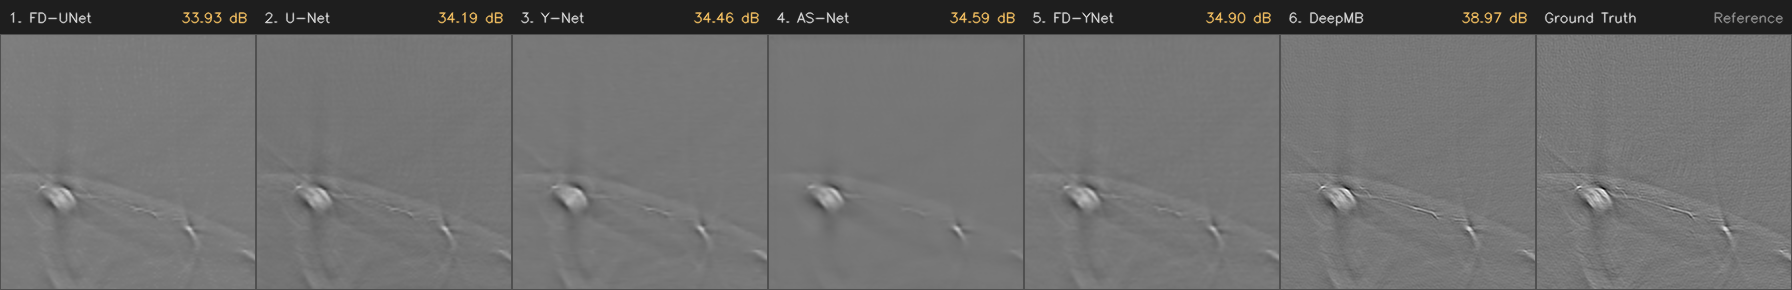
\includegraphics[width=0.95\textwidth]{sample2_comparison_grid.png}
\vspace{-2pt}
\caption{Visual comparison of Ground Truth and the six reconstruction methods.}
\label{fig:comparison}
\end{figure}

\vspace{5pt}
\begin{wraptable}{r}{0.48\textwidth}
\vspace{-15pt}
\centering
\caption{PSNR and SSIM Comparison (128 Sensors).}
\label{tab:metrics_comparison}
\fontsize{8}{9}\selectfont
\begin{tabular}{lcc}
\toprule
\textbf{Model} & \textbf{PSNR (dB)} & \textbf{SSIM}\\
\midrule
DeepMB & 38.97 & 0.9154\\
AS-Net & 36.86 & 0.8901\\
FD-YNet & 34.90 & 0.8291\\
Y-Net & 34.46 & 0.8131\\
U-Net & 34.19 & 0.8426\\
FD-UNet & 33.93 & 0.8411\\
\bottomrule
\end{tabular}
\vspace{-10pt}
\end{wraptable}

Table 1 summarizes the quantitative comparison. DeepMB achieves the highest PSNR by preserving measurement-domain information throughout the reconstruction pipeline. FD-YNet, AS-Net, and Y-Net achieve competitive intermediate performance by utilizing dual-input feature fusion and joint measurement-domain learning. Conversely, U-Net records a lower PSNR, experiencing smoothing that can affect fine structural details. The visual comparison in Fig.1 supports these quantitative findings.

The results indicate that incorporating imaging physics into the reconstruction pipeline substantially improves sparse-view PAT performance. Physics-guided learning preserves structural information more effectively than purely image-domain enhancement, while dense feature reuse offers an efficient alternative with competitive reconstruction quality. Future work will focus on improving dual-input architectures through multi-scale feature learning and better measurement-domain fusion.

\vspace{10pt}
{\fontsize{8}{9}\selectfont
\textbf{References}\\[2pt]

[1] Ko-Tsung Hsu, Steven Guan, and Parag V. Chitnis, ``Comparing deep learning frameworks for photoacoustic tomography image reconstruction,'' \textit{Photoacoustics}, vol. 23, p. 100271, 2021.

[2] Mengjie Guo, Hengrong Lan, Changchun Yang, and Fei Gao, ``AS-Net: Fast Photoacoustic Reconstruction with Multi-feature Fusion from Sparse Data,'' \textit{IEEE Transactions on Computational Imaging}, vol. 7, pp. 1180--1192, 2021.

[3] Christoph Dehner, Guillaume Zahnd, Vasilis Ntziachristos, and Dominik Jüstel, ``DeepMB: Deep neural network for real-time optoacoustic image reconstruction with adjustable speed of sound,'' \textit{Medical Image Analysis}, vol. 84, p. 102715, 2023.

[4] F. Ozdemir, B. Lafci, X. L. Deán-Ben, D. Razansky, and F. Perez-Cruz, ``OADAT: Experimental and Synthetic Clinical Optoacoustic Data for Standardized Image Processing,'' \textit{Transactions on Machine Learning Research (TMLR)}, 2023.
}

\end{document}